\chapter{Assoziationsdatenbank und API}
Das Ziel von TIMA ist das Erstellen einer Datenbank, in denen Assoziation gespeichert werden. Daher liegt ein Schwerpunkt unserer Arbeit darin, diese zu Erstellen und zu Befüllen. Die Datenbank ist direkt verknüpft mit einem Webfrontend, das durch die Bereitstellung einer umfassenden API der Hauptanlaufpunkt für die Benutzer und die Apps ist.

In diesem Kapitel werden das Backend der Webseite und die Datenbank beschrieben. Dabei wird genauer auf die Designentscheidungen eingangen, die zum Aufbau der einzelnen Datenbankbestanteile geführt haben.

\section{Backend und Datenbank}
Für das Backend der Website haben wir uns für Django als grundlegende Bibliothek entschieden. Bei Django handelt es sich um ein in Python geschriebenes Webframework, das dem Model-View-Controller-Schema folgt. Django bietet unter anderem einen sehr komplexen objektrelationalen Mapper, der es ermöglicht auch komplexe Objektstrukturen abzubilden ohne die verwendete Datenbank explizit zu kennen. Neben allen notwendigen Funktionen gewährleistet Django zusätzlich also gute Wiederverwendbarkeit und wurde deshalb für das Erstellen des Backends genutzt.

\subsection{Datenmodell}
In \hyperref[fig:uml]{Abbildung \ref*{fig:uml}} ist das komplette Datenmodell von TIMA dargestellt. Das Modul \texttt{associations.models} spielt dabei die Schlüsselrolle. Hier werden die grundlegenden Daten für die Assoziationsdatenbank gespeichert: die Worte und deren Verknüpfungen.

\begin{figure}
	\centering
	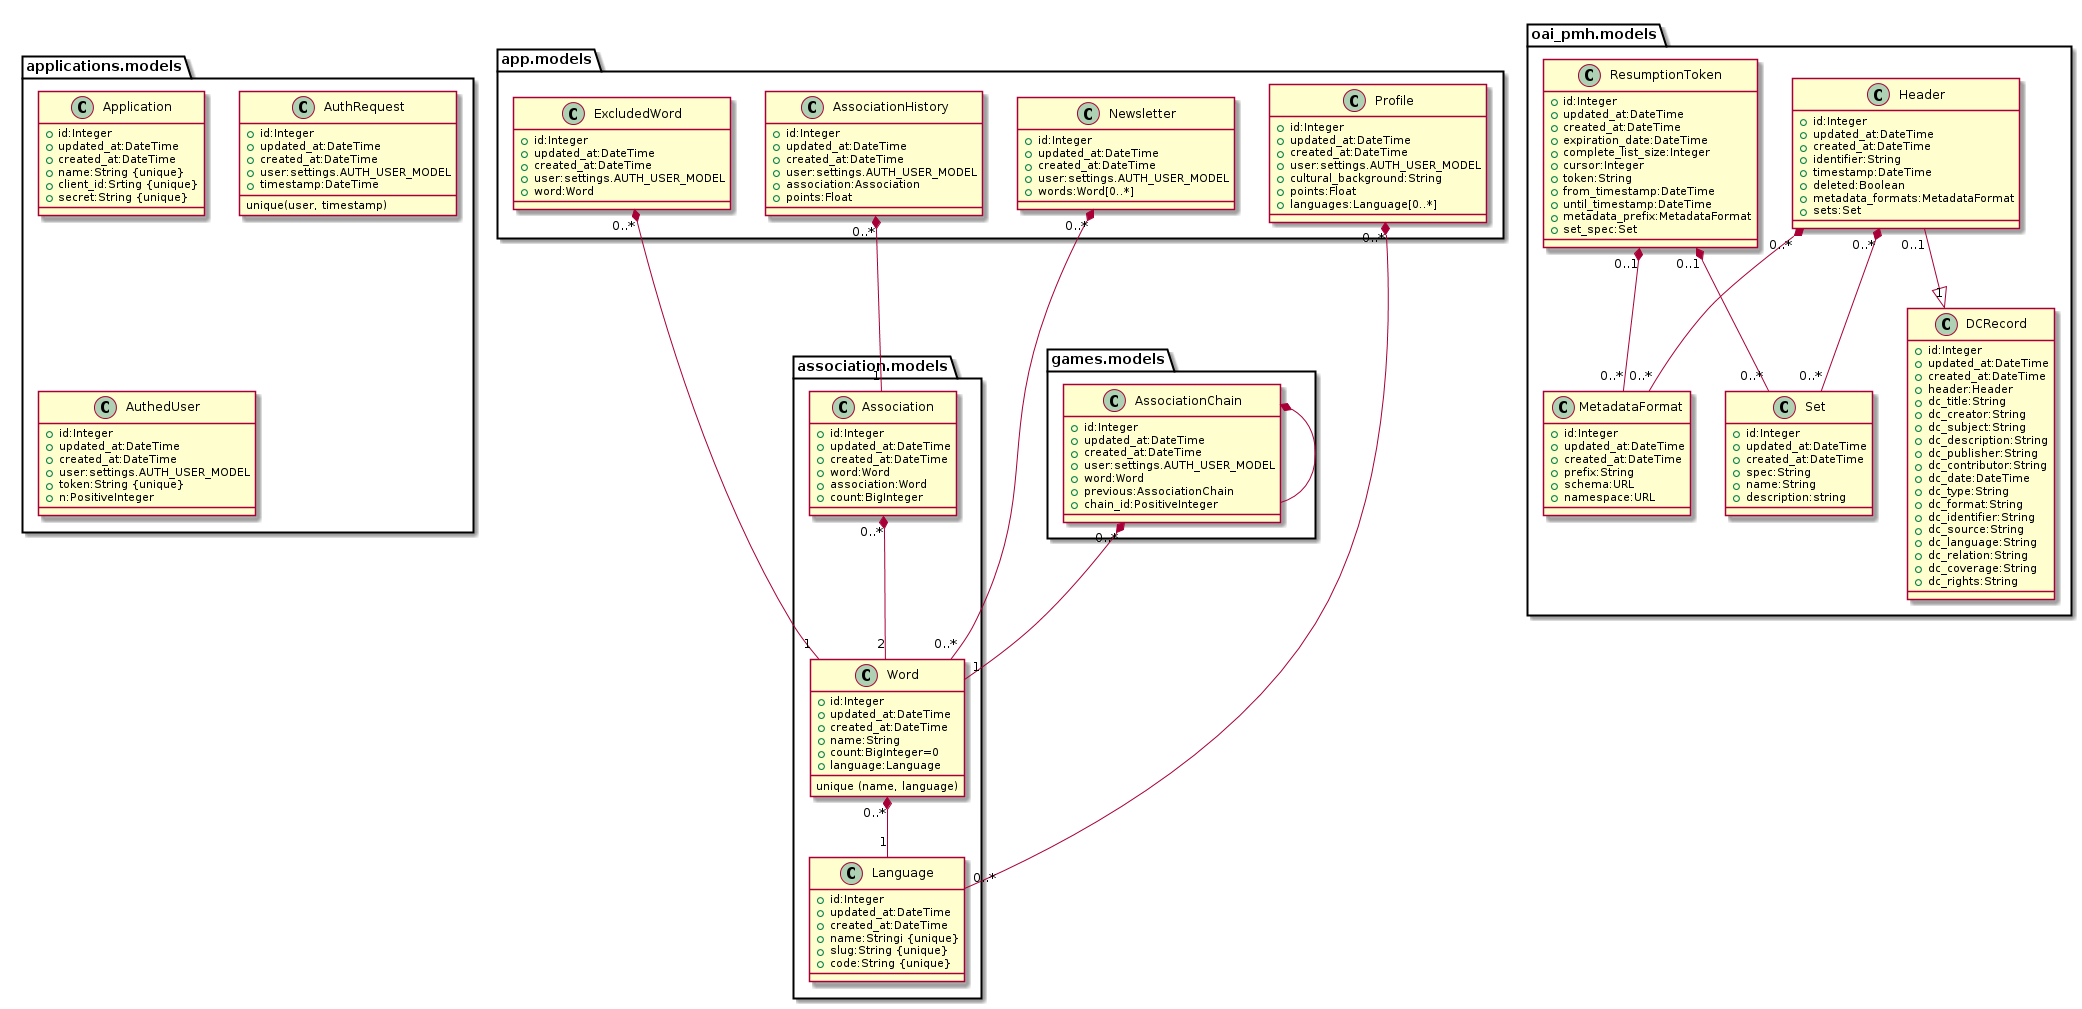
\includegraphics[width=\textwidth]{images/uml.png}
	\caption{UML des TIMA Datenmodells}
	\label{fig:uml}
\end{figure}

Das Modell \texttt{Word} speichert einzelne Wörter und das Modell \texttt{Association} die Assoziationen zwischen diesen Wörtern. Für jedes Wort wird gespeichert, wie oft für dieses nach einer Assoziation gefragt wurde. In ähnlicher Weise besitzt auch jede Assoziation in der Datenbank eine Häufigkeit, die angibt wie oft die Assoziation von Nutzern eingegeben wurde.
Um eine Unterscheidung zwischen verschiedenen Sprachen zu ermöglichen, repräsentiert das Modell \texttt{Language} die verfügbaren Sprachen. Existiert ein Wort in mehreren Sprachen oder wird in verschiedenen Sprachen genutzt, hat es für jede Sprache einen eigenen Eintrag.
\newline

Das Modul \texttt{games.models} enthält Modelle die für die verschiedenen Spiele wichtig sind. Dies ist im Moment nur AssoziationsKette (vgl. \hyperref[subsec:games]{Abschnitt \ref*{subsec:games}}), hierfür werden in dem Modul \texttt{AssociationChain} die letzte beziehungsweise aktuelle Assoziationskette eines Benutzer gespeichert. Diese wird beim Start eines neuen Spieles gelöscht.
\newline


Um grundlegende Funktionen des Benutzermanagements zu ermöglichen, wurden die Modelle des Moduls \texttt{app.models} eingeführt. Das Modell \texttt{Profile} speichert grundlegende Informationen zu jedem Nutzer, zum Beispiel die Punktzahl und die Sprachen, für die ein Benutzer assoziiert hat. Diese Daten werden in einem Ranglistensystem genutzt, das die Nutzer motivieren soll, sich gegenseitig zu messen. In dem Modell \texttt{AssociationHistory} wird die gesamte Assoziationsgeschichte eines Benutzers gespeichert, mit den jeweils für eine Assoziation erhaltenen Punkte. Somit können im Falle eines Misbrauchs die gegebenen Assoziationen aus der Datenbank gelöscht werden und dem Nutzer die Punkte entzogen werden.
Das Modell \texttt{ExcludeWord} enthält für jeden Benutzer die Wörter, die er innerhalb der letzten sieben Tage übersprungen hat (vgl. \hyperref[subsec:excludewords]{Abschnitt \ref*{subsec:excludewords}}). Das letzte Modell in diesem Modul speichert für jeden Benutzer welche Worte er in seinem Newsletter empfangen möchte.
\newline

Für die Kommunikation zwischen App und Backend, insbesondere der Autorisierung der Schreibzugriffe auf die Datenbank (vgl. \hyperref[sec:api]{Abschnitt \ref*{sec:api}}) dient das Modul \texttt{applications.models}. Das Modell \texttt{Application} speichert die Apps, die Autorisiert sind, mit den nötigen Daten für die Autorisierung (vgl. \hyperref[subsec:autorisierte_anfragen]{Abschnitt \ref*{subsec:autorisierte_anfragen}}). Die beiden anderen Modelle dieses Moduls \texttt{AuthRequest} und \texttt{AuthedUser} speichern die nötigen Information für einen Benutzer der sich authentifizieren möchte oder sich bereits authentifiziert hat. Durch dieses Modul wird also gewährleistet, dass nur Nutzer auf die Datenbank zugreifen können, die eine von uns autorisierte Anwendung nutzt.
\newline

Das letzte Modul und die beinhalteten Modell sind für das OAI-PMH erforderlich siehe dafür (vgl. \hyperref[sec:oai-pmh]{Abschnitt \ref*{sec:oai-pmh}}).


\section{API}\label{sec:api}
Damit verschiedene Apps mit der TIMA Datenbank kommunizieren können, haben
wir uns entschieden eine umfangreiche API zu implementieren. Diese lässt sich
grob in drei Teile gliedern. Zum einen gibt es die Anfragen, die keiner
Autorisierung bedürfen, zweitens jene die einer Autorisierung erfordern und
drittens eine OAI-PMH Schnittstelle.

Eine komplette Dokumentation der API ist in der Datei API.md\footnote{\url{https://github.com/Tima-Is-My-Association/TIMA/blob/master/API.md}} im git zu finden.

Im folgenden Abschnitt werden die einzelnen API Anfragen erläutert, zuerst die autorisierungsfreien, dann jene, die eine Autorisierung benötigen. Zum Schluss wird dann noch ein Abschnitt zu OAI-PMH folgen.

\subsection{Nicht autorisierte Anfragen}
Die API-Anfragen, die keiner Autorisierung bedürfen sind allgemeine Anfragen, an die Assoziationsdatenbank, die auch über die Webseite ohne eine Anmeldung erfolgen können.

\paragraph{Rangliste} Eine dieser Anfragen ist die nach der Rangliste. Es werden keine weiteren Angaben benötigt und als Antwort kommt ein JSON-Object, das eine Liste der Benutzer enthält, mit den gleichen Daten wie sie über die Webseite einsehbar sind.

\paragraph{Statistik} Ebenso ist die Statistik über die API abfragbar. Diese enthält aktuelle Zahlen über Nutzerzahl, Wortmenge und Assoziationen in der Datenbank.

\paragraph{Sprachen} Es kann eine Liste aller Sprachen in TIMA angefordert werden, hier ist neben dem Namen, der Sprach-Code in der Antwort enthalten, der bei vielen anderen Anfragen als Parameter angegeben werden muss.

\paragraph{Wörter} Um entweder ein einzelnes Wort oder eine Liste von Wörtern ist diese Anfrage bestimmt. Es können optional Wort-IDs, Sprache oder ein Limit für die Anzahl der Assoziationen pro Wort angegeben werden. Das JSON-Objekt der Antwort enthält unter anderem zu jedem Wort einen Link zur Website des Wortes, ein Link zu dieser Anfrage mit der Auswahl auf das einzelne Wort und der OAI-PMH identifier des Wortes.

\subsection{Autorisierte Anfragen}\label{subsec:autorisierte_anfragen}
Autorisierte Anfragen sind notwendig, um Schreibzugriff auf die Datenbank zuzulassen. Außerdem ist eine Authentisierung notwendig, um Nutzer der App oder der Webseite eindeutig identifizieren zu können. Für die Rangliste ist das unumgänglich. Aus diesem Grund war es erforderlich, dass einige API Anfragen einer Autorisierung bedürfen.

Um dies zu realisieren haben wir uns zunächst bestehende Frameworks wie zum Beispiel OAuth2 angeschaut und getestet in wie weit diese unseren Anforderungen genügen. Dies hat allerdings zu keinen zufriedenstellendem Ergebnis geführt, weswegen wir entschieden haben dies selbstständig zu implementieren.

Die grundlegenden Anforderungen die wir dabei hatten sind wie folgt:
\begin{enumerate}
	\item Sichere Authentisierung einer App
	\item Sichere Authentisierung eines Benutzers
	\item Sicherstellen, das spätere Anfragen von einem authorisierten Benutzer kommen
\end{enumerate}

\begin{figure}[!h]
	\centering
	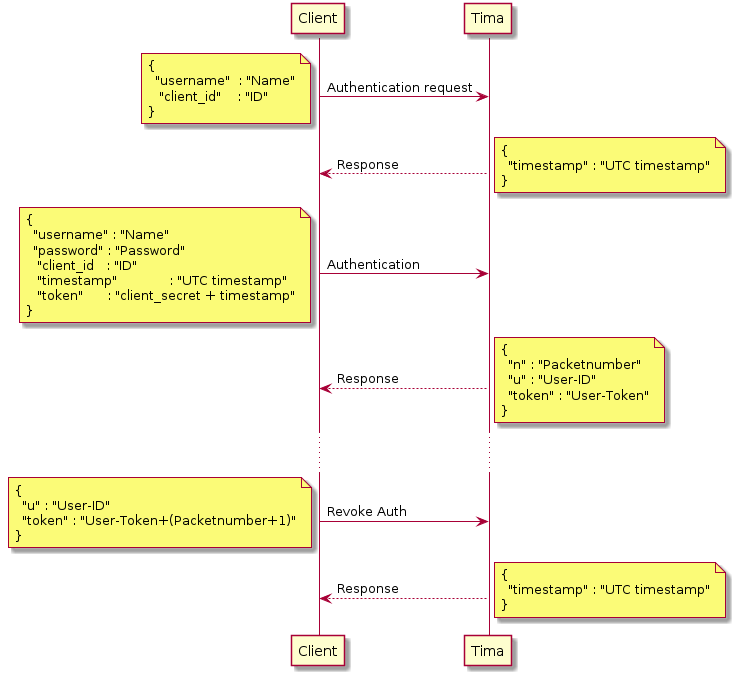
\includegraphics[width=\textwidth]{images/auth.png}
	\caption{Authentisierungsprozess}
	\label{fig:auth}
\end{figure}

In \hyperref[fig:auth]{Abbildung \ref*{fig:auth}} ist der Authentisierungsprozess schematisch Dargestellt. Der Client ist dabei eine App, über die sich ein Nutzer authentisieren möchte. Die App verfügt zum einen über eine \texttt{client\_id} und über ein \texttt{secret}, beides von TIMA vergebene eindeutige zufällige Strings. Der Authentisierungsprozess läuft wie folgt ab:
\begin{enumerate}
	\item Eine App sendet eine Anfrage an TIMA mit dem \texttt{username} des Benutzers und der \texttt{client\_id}. TIMA prüft diese beiden Werte auf Existenz und antwortet entweder mit \textbf{200} (HTTP Response Code) und dem aktuellen Zeitstempel oder mit \textbf{404}.
	\item Als nächstes sendet die App die eigentliche Authentisierungsanfrage. Mit \texttt{username} und \texttt{password} des Benutzers, \texttt{client\_id} der App, dem Zeitstempel der Antwort der letzten Anfrage und einem \texttt{token} das aus dem \texttt{secret} der App und dem Zeitstempel geniert wird (SHA512).
	\item TIMA antwortet wenn die Authentisierung erfolgreich war mit \textbf{200} und den folgenden drei Werten:
	\begin{itemize}
		\item[n] Paketnummer - jede Anfrage einer App muss diese um eins nach oben zählen. Als Wertebereich ist uint32 zubenutzen.
		\item[u] eine eindeutige Benutzer-ID, die bei jeder Anfrage mit zusenden ist
		\item[token] ein zufälliger String, der bei jeder Anfrage zusammen mit \texttt{n}, der Paketnummer, in einem SHA512 Hash zu senden ist
	\end{itemize}
\end{enumerate}

Aus Kompatibilitätsgründen läuft die Paketnummer im wertebereich uit32, also bis maximal 2147483646, und fängt nach erreichen der Maximalzahl wieder bei 0 an. Dies führt jedoch bei momentanen Nutzerzahlen zu keinen Problemen und wird mit sehr hoher Wahrscheinlich auch in Zukunft kein Thema werden.

\subsection{OAI-PMH}\label{sec:oai-pmh} %FIXME: Wofür?
Bei OAI-PMH (Open Archives Initiative - Protocol for Metadata Harvesting) handelt es sich um ein auf XML basierendes Protokoll zum Sammeln von Metadaten. Es wird dabei unterschieden zwischen Data Providern und Service Providern. Ein Data Provider betreibt ein oder mehrere Repositories, die OAI-PMH unterstützen um Metadaten bereitzustellen. Service Provider sammeln die Metadaten der Data Providern und bieten Mehrwertdienste an.

Wir haben das OAI-PMH Protokoll implementiert um Metadaten zu den gesammelten Assoziationen bereitzustellen. Wir stellen dabei Metadaten zu den Wörtern und im geringen Maße zu den Benutzern bereit.